\documentclass[a4paper]{article}

\usepackage{fullpage}
\usepackage{caption}
\usepackage{tikz}
\usetikzlibrary{trees,backgrounds}

\title{Treatment categorization: deciding when treatments should be considered distinct for the purpose of analysis}
\date{}

\begin{document}

\maketitle

\section{Purpose}

In ADDIS, the study design information of a clinical trial should match what happened in reality as closely as possible.
For example, if patients were administered Fluoxetine, for which the dose could be titrated from 20 mg/day to 40 mg/day, this should be modelled explicitly as ``treatment with Drug(Fluoxetine) at FlexibleDose(20 mg/day -- 40 mg/day)''.
That way, different studies including Fluoxetine can unambiguously be identified as such.
Importantly, the data that is entered for a study should be independent of any specific analysis, to allow reuse of the data for different analyses.

However, when performing a meta-analysis, we require crisp definitions of which treatments should be considered distinct for the analysis.
In additions, these definitions may differ between analyses.
For example, we might be performing a meta-analysis between Fluoxetine and Paroxetine, and not care about the specific dose.
On the other hand, we might also be interested in the effect of `high dose' Fluoxetine compared to that of `low dose' Fluoxetine.
This requires the classification, or categorization, of the arms that include Fluoxetine into two discrete and mutually exclusive categories.

One solution would be to enter two drugs, `Fluoxetine low dose' and `Fluoxetine high dose' and use these in the study design definitions as appropriate.
However, this violates the principle of analysis independence for the study data.
Thus, a different solution is needed that allows us to flexibly define treatment categories for the purpose of analysis.

\section{Handling dose information}

Dose information can be handled in many different ways in meta-analysis.
The way it is currently handled in ADDIS is that dose information is ignored completely.
If the user wishes to take the dose into account, this can be achieved by including and excluding studies and/or arms.
An alternative would be to perform a meta-regression taking into account the dose as a covariate.
We could (instead or in addition) define a range of `typical' or `acceptable' doses and include only studies that adhere to this range.
Finally, we might want to view several ranges of dose as distinct treatments, e.g. comparing `low dose' and `high dose' variants of a drug.
Notice that including the dose as a covariate in the analysis and constructing definitions of which (drug, dose) combinations should be considered `the same' for the purpose of analysis are largely orthogonal issues.
Therefore, we will only consider the categorization of (drug, dose) combinations for the present discussion.

\section{Treatment categorization}

Given a specific drug, we want to separate different doses into mutually exclusive categories.
In some cases, these categories might be exhaustive, but in others we might want to not consider (exclude from the analysis) some doses.
In the following, several examples of possible decision trees will be given.

The current situation in ADDIS is as follows:

\begin{center}
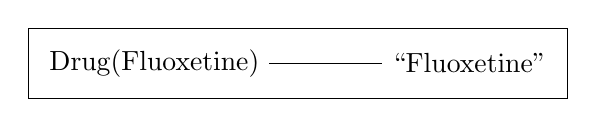
\begin{tikzpicture}[grow=right, sloped, level distance=4cm, framed]
\node {Drug(Fluoxetine)}
	child { node {``Fluoxetine''} };
\end{tikzpicture}
\captionof{figure}{Categorization: Fluoxetine (any dose)}
\end{center}

If we consider only fixed dose studies for the moment, we might want to restrict the dose to the range of licensed doses:

\begin{center}
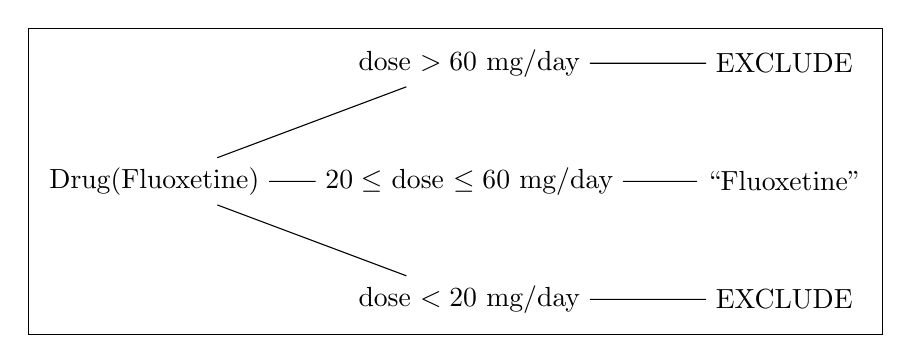
\begin{tikzpicture}[grow=right, sloped, level distance=4cm, framed]
\node {Drug(Fluoxetine)}
	child { node {dose $< 20$ mg/day} child { node {EXCLUDE} }}
	child { node {$20 \leq$ dose $\leq 60$ mg/day} child { node {``Fluoxetine''} }}
	child { node {dose $> 60$ mg/day} child { node {EXCLUDE} }};
\end{tikzpicture}
\captionof{figure}{Categorization: Fluoxetine (licensed dose)}
\end{center}

Furthermore, we might want to distinguish high and low dose:

\begin{center}
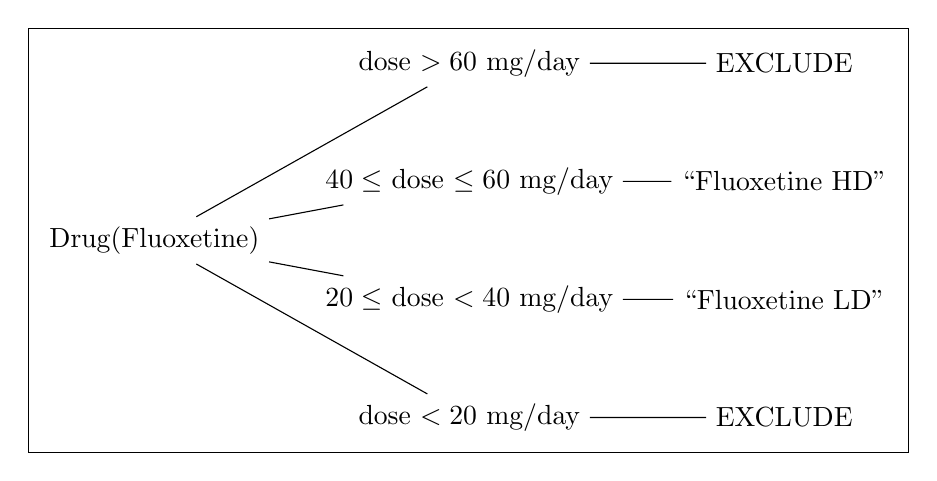
\begin{tikzpicture}[grow=right, sloped, level distance=4cm, framed]
\node {Drug(Fluoxetine)}
	child { node {dose $< 20$ mg/day} child { node {EXCLUDE} }}
	child { node {$20 \leq$ dose $< 40$ mg/day} child { node {``Fluoxetine LD''} }}
	child { node {$40 \leq$ dose $\leq 60$ mg/day} child { node {``Fluoxetine HD''} }}
	child { node {dose $> 60$ mg/day} child { node {EXCLUDE} }};
\end{tikzpicture}
\captionof{figure}{Categorization: Fluoxetine HD/LD}
\end{center}

In general, we will also have to take into account the type of dosing:

\begin{center}
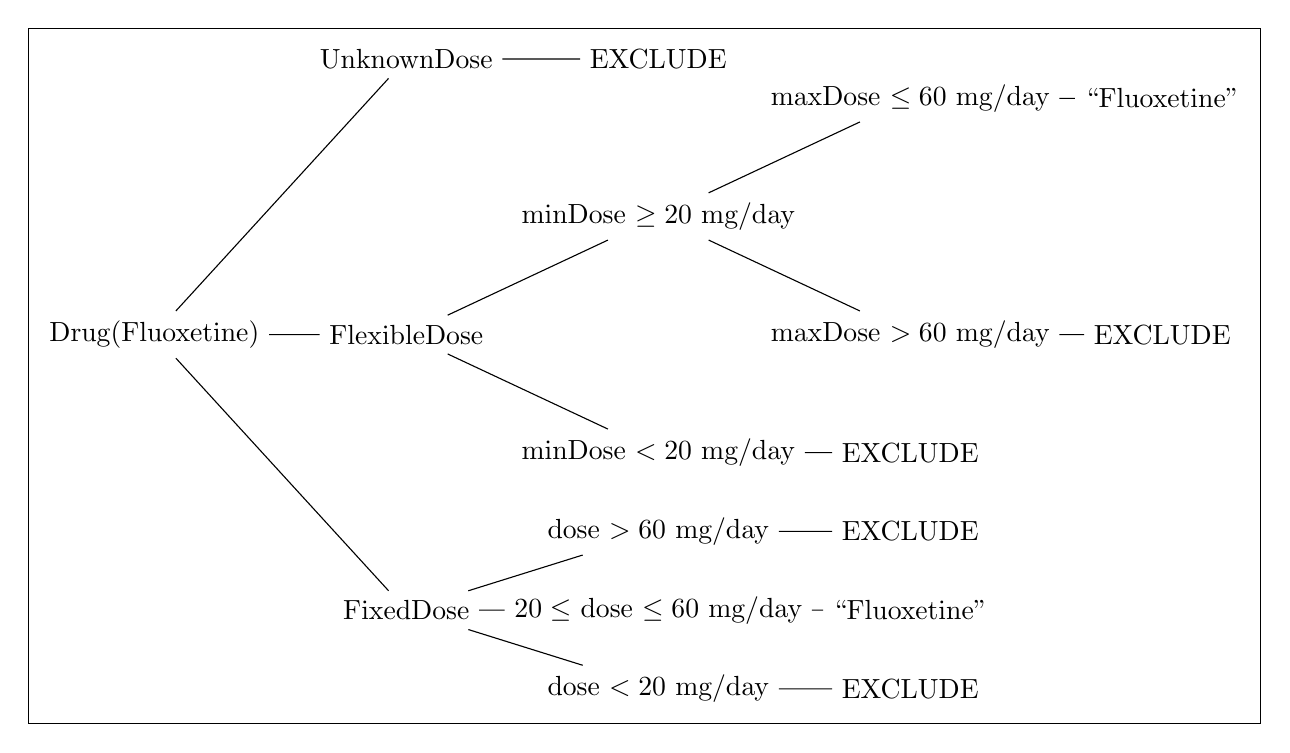
\begin{tikzpicture}[grow=right, level distance=3.2cm, framed]
\node {Drug(Fluoxetine)} [sibling distance=3.5cm]
	child { node {FixedDose} [sibling distance=1cm]
		child { node {dose $< 20$ mg/day} child { node {EXCLUDE} }}
		child { node {$20 \leq$ dose $\leq 60$ mg/day} child { node {``Fluoxetine''} }}
		child { node {dose $> 60$ mg/day} child { node {EXCLUDE} }}
	}
	child { node {FlexibleDose} [sibling distance=3cm]
		child { node {minDose $< 20$ mg/day} child { node {EXCLUDE} }}
		child { node {minDose $\geq 20$ mg/day}
			child { node {maxDose $> 60$ mg/day} child { node {EXCLUDE} }}
			child { node {maxDose $\leq 60$ mg/day} child { node {``Fluoxetine''} }}
		}
	}
	child { node {UnknownDose} child { node {EXCLUDE} }};

\end{tikzpicture}
\captionof{figure}{Categorization: Fluoxetine (licensed dose)}
\end{center}

The decision tree framework allows for fully flexible handling of dose information, but may not be the most convenient for common use cases.
We might want to provide `default' decision trees for some common situations (e.g. ignoring dose information or limiting the dose to a specific range).

\subsection{Scope of categorizations}

Then there is the status of these `categorizations' to consider.
First of all, each dose categorization applies only to a single drug, since the potency of drugs varies greatly.
Secondly, should they be fully local to a single meta-analysis, or should they be shared between analyses?
The first option is cumbersome: a new decision tree would have to be created for each analysis, while it is likely that several analyses will be created based on the same definitions.
Moreover, to enable benefit-risk analysis, the same categorizations have to be used {\em between} analyses.
Thus, the per-meta-analysis option is not realistic.
Ideally, we might want to create an `analysis context' within which specific categorizations are defined.
However, to keep it simple, we can store a global collection of categorizations, and let the user choose the most appropriate one (for each drug) in the meta-analysis wizard.

\subsection{Dealing with combination treatments}

Now that we can define categories within a specific drug, the question is how to generalize to combinations of drugs.
There are several possible approaches, but only one if we consider that statistical modelling of combination treatments (see Welton et al., Am J Epidemiol, 2009) needs to be possible.
To enable this, we must apply the categorizations per-drug, giving rise to combinations of categories.
For example, if for Fluoxetine we have ``Fluoxetine LD'' and ``Fluoxetine HD'' and for Paroxetine we have ``Paroxetine LD'' and ``Paroxetine HD'', there will be four distinct combination treatments:
\begin{itemize}
\item ``Fluoxetine LD'' + ``Paroxetine LD''
\item ``Fluoxetine LD'' + ``Paroxetine HD''
\item ``Fluoxetine HD'' + ``Paroxetine LD''
\item ``Fluoxetine HD'' + ``Paroxetine HD''
\end{itemize}
The user can then include/exclude combinations according to his own interest, but there is only a single definition of the categories that applies to both combination treatments and single treatments.

Note that we do not consider the `lumping' of drugs: it is not possible to have a certain group of drugs categorized as the same treatment, nor is it possible to have certain drugs ignored when they occur in combination with another drug (e.g. `Fluoxetine' and `Fluoxetine + Paroxetine' to be considered the same).
In general these analysis strategies, while quite commonly used, are not defensible, and better alternatives (network meta-analysis and statistical modelling of combination treatments) are available.

\section{Conclusion}

Defining categorizations of doses within a specific drug allows us to flexibly define treatments for the purposes of analysis, without compromising the analysis-independence of the study data.
Moreover, by considering the dose only per-drug, we keep the path to statistical modelling of combination treatments open and keep user workload to a minimum.
Finally, we decided against incorporating treatment definitions that go across drugs due to questionable validity of the potential use cases.

\end{document}
